\section{Zielsetzung und Nutzen (Benefits)}
Ziel des Grobkonzepts ist es, eine vollständig automatisierte Anlage zu entwickeln. Diese soll die aktuell noch manuell durchgeführten Tätigkeiten zur Verpackung der Bremssysteme vollständig als eigenständig integriertes System ablösen.\\
Durch die Implementierung einer solchen automatisierten Anlage soll der Gesamtprozess effizienter gestaltet werden. Ein weiteres Ziel ist die Sicherstellung einer gleichbleibend hohen Verpackungsqualität. Somit werden Engpässe im Produktionsfluss vermieden und die Anlagenverfügbarkeit steigt.\\\\
Ein zentrales Ziel besteht darin, die Zykluszeit zu verringern und damit den Durchsatz\footnote{Der Durchsatz beschreibt die Anzahl der produzierten Einheiten pro Zeiteinheit.} zu erhöhen. Somit kann langfristig eine Gewinnmaximierung erzielt werden. Zudem soll das System eine reproduzierbare Verpackungsqualität gewährleisten und somit Fehlereinflüsse, die durch manuelle Bearbeitung entstehen, vermeiden.\\\\
Neben den technischen Vorteilen gibt es auch wirtschaftliche Aspekte, die für eine Umsetzung sprechen. Der Personalbedarf kann deutlich reduziert werden, wodurch eine langfristige Kostensenkung gewährleistet ist. Gleichzeitig werden die Mitarbeitenden körperlich entlastet und können künftig in höherwertigen Tätigkeitsfeldern eingesetzt werden. Dies führt zu einer gesteigerten Motivation und einer besseren Qualifizierung.
\begin{figure}[H]
	\centering
	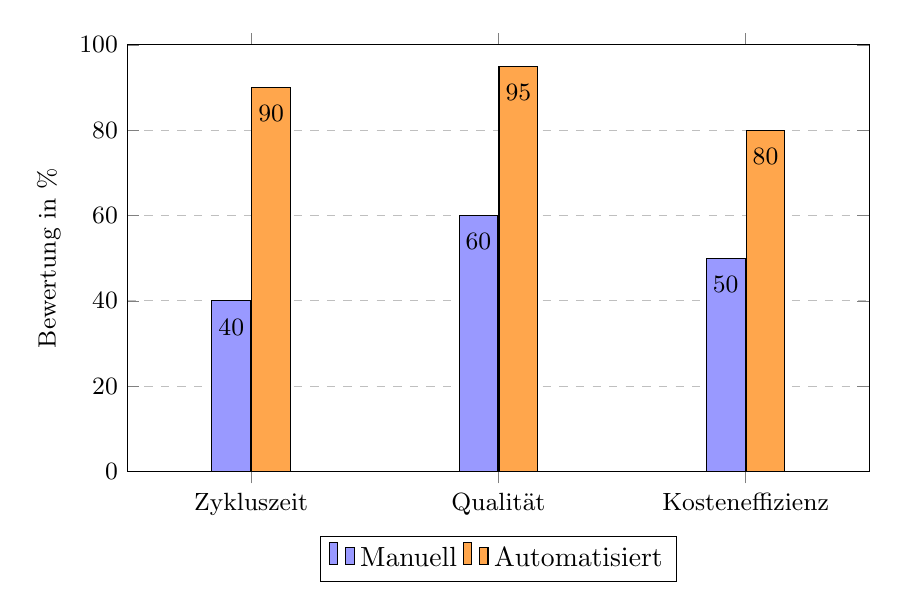
\begin{tikzpicture}
		\begin{axis}[
			ybar=0.4,
			bar width=14pt,
			width=11cm,
			height=7cm,
			enlarge x limits=0.25,
			ymin=0, ymax=100,
			ylabel={Bewertung in \%},
			symbolic x coords={Zykluszeit,Qualität,Kosteneffizienz},
			xtick=data,
			nodes near coords,
			every node near coord/.append style={
				font=\small,
				anchor=north,   % Text zeigt nach unten
				yshift=-3pt     % leicht nach unten verschoben
			},
			legend style={at={(0.5,-0.15)},anchor=north,legend columns=-1},
			ymajorgrids=true,
			grid style=dashed,
			tick label style={font=\small},
			label style={font=\small},
			]
			
			% --- Daten: Manuell ---
			\addplot[fill=blue!40] coordinates {
				(Zykluszeit,40)
				(Qualität,60)
				(Kosteneffizienz,50)
			};
			
			% --- Daten: Automatisiert ---
			\addplot[fill=orange!70] coordinates {
				(Zykluszeit,90)
				(Qualität,95)
				(Kosteneffizienz,80)
			};
			
			\legend{Manuell, Automatisiert}
		\end{axis}
	\end{tikzpicture}
	\caption{Vergleich der Hauptnutzen der Automatisierung gegenüber dem manuellen Verpackungsprozess}
	\label{fig:nutzenvergleich}
\end{figure}




Wie in Abbildung \ref{fig:nutzenvergleich} dargestellt, ergeben sich durch die Automatisierung deutliche Vorteile in allen relevanten Bereichen. Besonders stark verbessert sich die Zykluszeit, was zu einem höheren Durchsatz und einer besseren Auslastung der Produktionslinie führt. Gleichzeitig steigt die Verpackungsqualität und die langfristigen Prozesskosten sinken deutlich. Diese Faktoren leisten gemeinsam einen wesentlichen Beitrag zur Effizienzsteigerung und zur Stärkung der Wettbewerbsfähigkeit des Unternehmens.
